\chapter{Réflexions autour de l'IA et limites de l'outil créé}
\label{chap:limites}

Le développement d'un outil de détection de fraude basé sur un agent IA, en assurance automobile constitue une avancée significative en matière d'aide à la décision. Néanmoins, son utilisation doit être appréhendée avec recul, tant sur le plan opérationnel que méthodologique, et ouvre plusieurs perspectives d'amélioration.

% --------------------------------------------------------------
\section{Un outil d'aide à la décision complémentaire avec l'humain}
% --------------------------------------------------------------

Il est encore une fois essentiel de souligner que l'agent IA ne se substitue pas au gestionnaire, mais s'inscrit dans une logique de \textbf{complémentarité homme-machine}. L'intervention humaine reste centrale à chaque étape du processus.

En amont, l'actuaire ou le \textit{data scientist} intervient dans la \textbf{construction et le paramétrage du modèle} : sélection de la base de données, choix du type de modèle (scoring en points, arbre de décision, Gradient Boosting), validation de sa performance et de sa cohérence métier.

En phase d'utilisation, le gestionnaire reste responsable de la \textbf{saisie des informations relatives au sinistre}, de l'interprétation du score fourni et, le cas échéant, de la décision finale d'investigation. Enfin, il contribue à l'amélioration continue du modèle en renseignant le \textbf{statut final du dossier (fraude ou non)}, après avoir fait lui-même l'enquête permettant de prouver cette réponse, alimentant ainsi la base d'apprentissage.

Les deux schémas ci-dessous illustrent concrètement les points d'intervention humaine au sein du processus : ils font apparaître, à chaque étape, la frontière entre ce que l'agent automatise et ce qui reste du ressort du gestionnaire.

\begin{figure}[H]
    \centering
    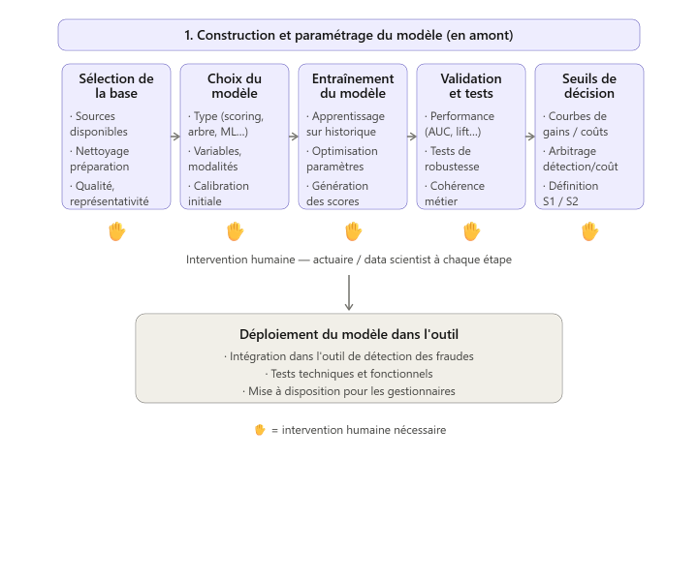
\includegraphics[width=0.9\textwidth]{images/chapitre7/schema_aide1.png}
    \caption{Points d'intervention humaine dans le module de construction du modèle}
    \label{fig:schema-aide1}
\end{figure}

\begin{figure}[H]
    \centering
    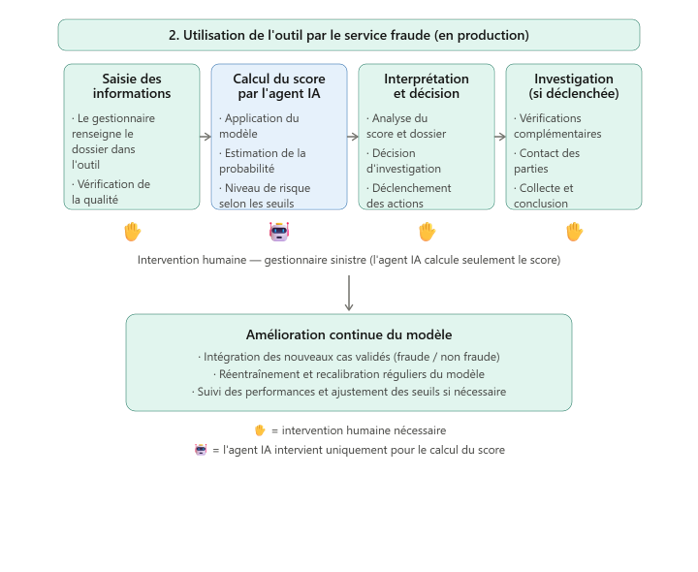
\includegraphics[width=0.9\textwidth]{images/chapitre7/schema_aide2.png}
    \caption{Points d'intervention humaine dans le module opérationnel de détection}
    \label{fig:schema-aide2}
\end{figure}

Ainsi, l'agent IA agit comme un outil d'aide à la décision structurant et homogénéisant, mais ne remplace en aucun cas l'expertise métier, indispensable pour interpréter les situations complexes et prendre des décisions adaptées.

% --------------------------------------------------------------
\section{Nature de l'IA utilisée : de l'IA générative à l'IA agentique}
% --------------------------------------------------------------

Il convient également de distinguer les différents types d'intelligence artificielle mobilisables dans ce contexte.

L'\textbf{IA générative} (comme les modèles de langage) est principalement utilisée pour produire du contenu (texte, code, synthèses) et assister dans des tâches d'analyse ou de documentation. À l'inverse, l'\textbf{IA agentique} s'inscrit dans une logique plus opérationnelle : elle est capable d'enchaîner des actions, de prendre des décisions simples et d'interagir avec un environnement en fonction d'objectifs définis.

En pratique, l'outil développé relève d'un \textbf{mélange de ces deux approches}, et il serait réducteur de le ranger dans une seule catégorie.

D'un côté, sa conception repose sur une logique largement \textbf{dirigée} : le raisonnement de l'agent a été décomposé, via le prompt, en une séquence d'étapes précises (ingestion, audit, analyse descriptive, modélisation, évaluation) que l'agent exécute dans l'ordre imposé. Sur ce plan, l'IA agit comme un exécutant guidé pas à pas, sans latitude sur l'enchaînement global de la tâche. Ce cadrage strict est d'ailleurs un choix assumé : il garantit la reproductibilité et l'auditabilité du dispositif, exigences essentielles dans un contexte assurantiel.

De l'autre, l'outil manifeste une véritable dimension \textbf{agentique} dans les décisions que l'agent prend de lui-même, sans instruction explicite, en mobilisant une logique métier ou statistique. Plusieurs exemples rencontrés au fil de ce mémoire l'illustrent : l'agent choisit seul la représentation graphique la plus adaptée à chaque variable (camembert pour un faible nombre de modalités, diagramme en barres au-delà) ; il détecte et écarte de lui-même les variables inexploitables, tels les identifiants uniques ou les variables trop granulaires ; il identifie le seuil de décision optimal via l'indice de Youden ; et il sélectionne, parmi les variables candidates, celles à retenir dans le barème de \textit{scoring}. Ces arbitrages, laissés à l'initiative de l'agent, constituent le cœur de son caractère agentique.

C'est cette combinaison qui caractérise l'outil : un cadre procédural dirigé, garant de rigueur et de traçabilité, au sein duquel l'agent conserve une autonomie de décision sur les choix méthodologiques et métiers.

À noter que par défaut, l'outil s'est initialement appuyé sur un \textbf{modèle de \textit{scoring} en points}, privilégié pour sa simplicité et son interprétabilité. Des extensions ont ensuite été introduites pour recourir à des modèles plus avancés, tels que les arbres de décision ou des méthodes de \textit{machine learning} comme le Gradient \textit{Boosting}. Le choix du modèle constitue lui-même un arbitrage entre interprétabilité et performance, décidé en fonction des besoins métiers.

% --------------------------------------------------------------
\section{Limites liées à la qualité et à la richesse des données}
% --------------------------------------------------------------

% --------------------------------------------------------------
\subsection{Le couplage à la base portefeuille}
% --------------------------------------------------------------

La performance et la pertinence d'un modèle de détection de fraude reposent de manière déterminante sur la qualité, la granularité et la richesse des données disponibles.

Dans le cadre de cette étude, le modèle est construit uniquement à partir d'une base sinistre, ce qui constitue une première limite importante. En effet, certaines informations structurantes issues de la base portefeuille ne sont pas accessibles, alors même qu'elles pourraient apporter un pouvoir explicatif significatif.

Parmi ces informations, on peut notamment citer l'ancienneté du contrat, l'historique de sinistralité de l'assuré, la fréquence de résiliation ou de souscription, ou encore des éléments d'identification permettant de reconstituer des liens entre individus (assurés, conducteurs, tiers).

Pour pallier partiellement cette limite, la base sinistre a été enrichie de trente variables reconstituant une partie de cette information (cf. section~\ref{sec:enrichissement}). Cet enrichissement ne remplace toutefois pas l'accès à une véritable base portefeuille, qui offrirait une profondeur historique et relationnelle hors de portée d'un enrichissement à partir du seul sinistre.

L'absence de ces variables limite la capacité du modèle à capter des comportements de fraude plus complexes, notamment ceux reposant sur des logiques de répétition ou d'organisation.

À titre d'exemple, en assurance automobile, l'accès à la base portefeuille permettrait de détecter plus efficacement certains schémas de fraude tels que :

\begin{itemize}[label = $\bullet$]
    \item \textbf{Fraudes opportunistes liées à une ancienneté très faible du contrat} : un sinistre survenant peu de temps après la souscription (ex : vol ou incendie dans les premières semaines) constitue un signal faible classique, difficile à exploiter sans information sur la date d'entrée en portefeuille.
    \item \textbf{Récurrence de sinistres sur un même assuré} : un assuré présentant une fréquence de sinistralité anormalement élevée sur une période donnée peut indiquer un comportement suspect (ex : déclarations répétées de bris de glace ou d'accidents matériels). Sans historique consolidé, ces signaux ne peuvent être captés que partiellement.
    \item \textbf{Stratégies de multi-assurance ou de résiliation stratégique} : certains fraudeurs peuvent multiplier les contrats auprès de différents assureurs ou résilier après sinistre pour éviter d'être détectés. L'analyse des trajectoires contractuelles (durée de détention, fréquence de changement d'assureur) constitue alors une variable explicative clé.
    \item \textbf{Fraudes en réseau ou en bande organisée} : l'identification de liens entre individus (même adresse, même véhicule impliqué dans plusieurs sinistres, tiers récurrents dans des accidents) permettrait de détecter des schémas de fraude structurés. Par exemple, des accidents impliquant régulièrement les mêmes personnes ou garages peuvent révéler des montages frauduleux (accidents simulés, complicités avec des réparateurs, etc.).
    \item \textbf{Incohérences entre profil assuré et sinistre déclaré} : certaines variables portefeuille (âge, ancienneté de conduite, historique de comportement) permettent de mieux contextualiser un sinistre. Par exemple, un assuré sans historique de sinistre déclarant soudainement un sinistre grave peut être analysé différemment d'un profil déjà sinistré.
\end{itemize}

L'intégration de ces données permettrait d'introduire de nouvelles variables explicatives à forte valeur ajoutée actuarielle, telles que :

\begin{itemize}[label = $\bullet$]
    \item des indicateurs de fréquence individuelle de sinistralité ;
    \item \textbf{Variables de durée en portefeuille} ;
    \item \textbf{Scores de comportement client} ;
    \item \textbf{Variables de réseaux (\textit{graph analytics}) identifiant des connexions entre dossiers}.
\end{itemize}

Ces enrichissements contribueraient à améliorer significativement la capacité de discrimination du modèle, en captant des dimensions aujourd'hui absentes, notamment les effets temporels et relationnels. En pratique, cela se traduirait par une meilleure séparation entre sinistres frauduleux et non frauduleux, et donc une optimisation des actions de détection.

Au-delà de la richesse des variables, la qualité des données constitue également un enjeu majeur. Les erreurs de saisie, les données manquantes ou encore les délais dans la confirmation des fraudes peuvent introduire des biais dans l'apprentissage du modèle. Par ailleurs, la fraude étant par nature un phénomène partiellement observé, la base d'apprentissage est susceptible de contenir un biais de sous-détection, certaines fraudes n'étant jamais identifiées comme telles.

Ainsi, l'amélioration de la détection de fraude passe non seulement par le choix des modèles, mais aussi (et surtout) par une stratégie d'enrichissement et de fiabilisation des données. Dans cette perspective, l'intégration de données portefeuille, voire de données externes ou mutualisées, constitue un levier essentiel pour renforcer la robustesse et la performance du dispositif.

% --------------------------------------------------------------
\subsection{Ajout de données externes}
% --------------------------------------------------------------

En complément à l'enrichissement par les données issues de la base portefeuille, le recours à des \textbf{sources de données complémentaires} constitue un levier majeur d'amélioration des modèles de détection de fraude. En effet, la fraude étant un phénomène complexe et évolutif, sa détection nécessite une approche multidimensionnelle intégrant des informations variées, parfois extérieures au strict périmètre assurantiel.

En premier lieu, l'exploitation de données externes ouvertes (\textit{open data}) peut permettre d'apporter un éclairage contextuel précieux. Par exemple, les données météorologiques peuvent être mobilisées afin de vérifier la cohérence entre les circonstances déclarées d'un sinistre et les conditions climatiques réelles (pluie, grêle, tempête).

De même, les données géographiques permettent d'identifier des zones à risque, notamment en matière de vol ou de vandalisme, et d'analyser la fréquence des sinistres dans certaines localisations. Enfin, les données socio-économiques locales peuvent contribuer à affiner la compréhension des comportements, en intégrant des variables de contexte telles que le niveau de revenu ou les caractéristiques du territoire.

Par ailleurs, lorsque cela est possible, l'intégration de données télématiques constitue un apport particulièrement structurant. Ces données, issues de capteurs embarqués ou d'applications mobiles, permettent de reconstituer le comportement de conduite (vitesse, accélérations, freinages, horaires d'utilisation) et d'évaluer la cohérence entre l'usage réel du véhicule et le sinistre déclaré. Ainsi, un sinistre survenu dans des conditions incompatibles avec les données de conduite enregistrées peut constituer un signal fort de fraude.

Les données issues des prestataires (réparateurs, experts, avocats) représentent également une source d'information à forte valeur ajoutée. L'analyse de leur historique d'intervention permet d'identifier des acteurs apparaissant de manière récurrente dans des dossiers suspects. Une surreprésentation de certains prestataires dans des sinistres à fort taux de fraude peut révéler des comportements anormaux, voire des complicités, et constitue ainsi un levier de détection des fraudes organisées.

En outre, l'exploitation des données textuelles non structurées, telles que les descriptions de sinistres ou les comptes rendus d'expertise, ouvre des perspectives intéressantes grâce aux techniques de traitement automatique du langage (NLP). L'analyse de ces textes permet de détecter des incohérences, des formulations atypiques ou des schémas linguistiques récurrents associés à des comportements frauduleux. Ces informations, difficilement exploitables dans une approche classique, enrichissent considérablement la capacité du modèle à capter des signaux faibles.

Une autre piste d'amélioration repose sur l'utilisation d'une approche réseau (\textit{graph analytics}). Cette méthodologie consiste à modéliser les relations entre les différents acteurs d'un sinistre (assurés, tiers, véhicules, adresses, prestataires) afin d'identifier des communautés ou des structures anormales. Elle permet notamment de détecter des schémas de fraude organisée, caractérisés par la répétition de certaines combinaisons d'acteurs ou de situations (typiquement, les mêmes individus impliqués dans plusieurs sinistres, les mêmes véhicules ou les mêmes adresses apparaissant de manière récurrente). Cette approche relationnelle dépasse la simple analyse individuelle des dossiers et offre une vision plus globale des phénomènes de fraude.

Enfin, la mise en place de dispositifs de mutualisation inter-assureurs constituerait un levier particulièrement puissant. Le partage d'informations, dans un cadre réglementaire adapté, permettrait de disposer d'un historique multi-compagnies et de détecter des comportements frauduleux dits « nomades », consistant pour un individu à reproduire des schémas de fraude auprès de différents assureurs. Une telle mutualisation renforcerait significativement la capacité de détection, en élargissant le périmètre d'observation et en limitant les angles morts propres à chaque compagnie.

\begin{figure}[H]
    \centering
    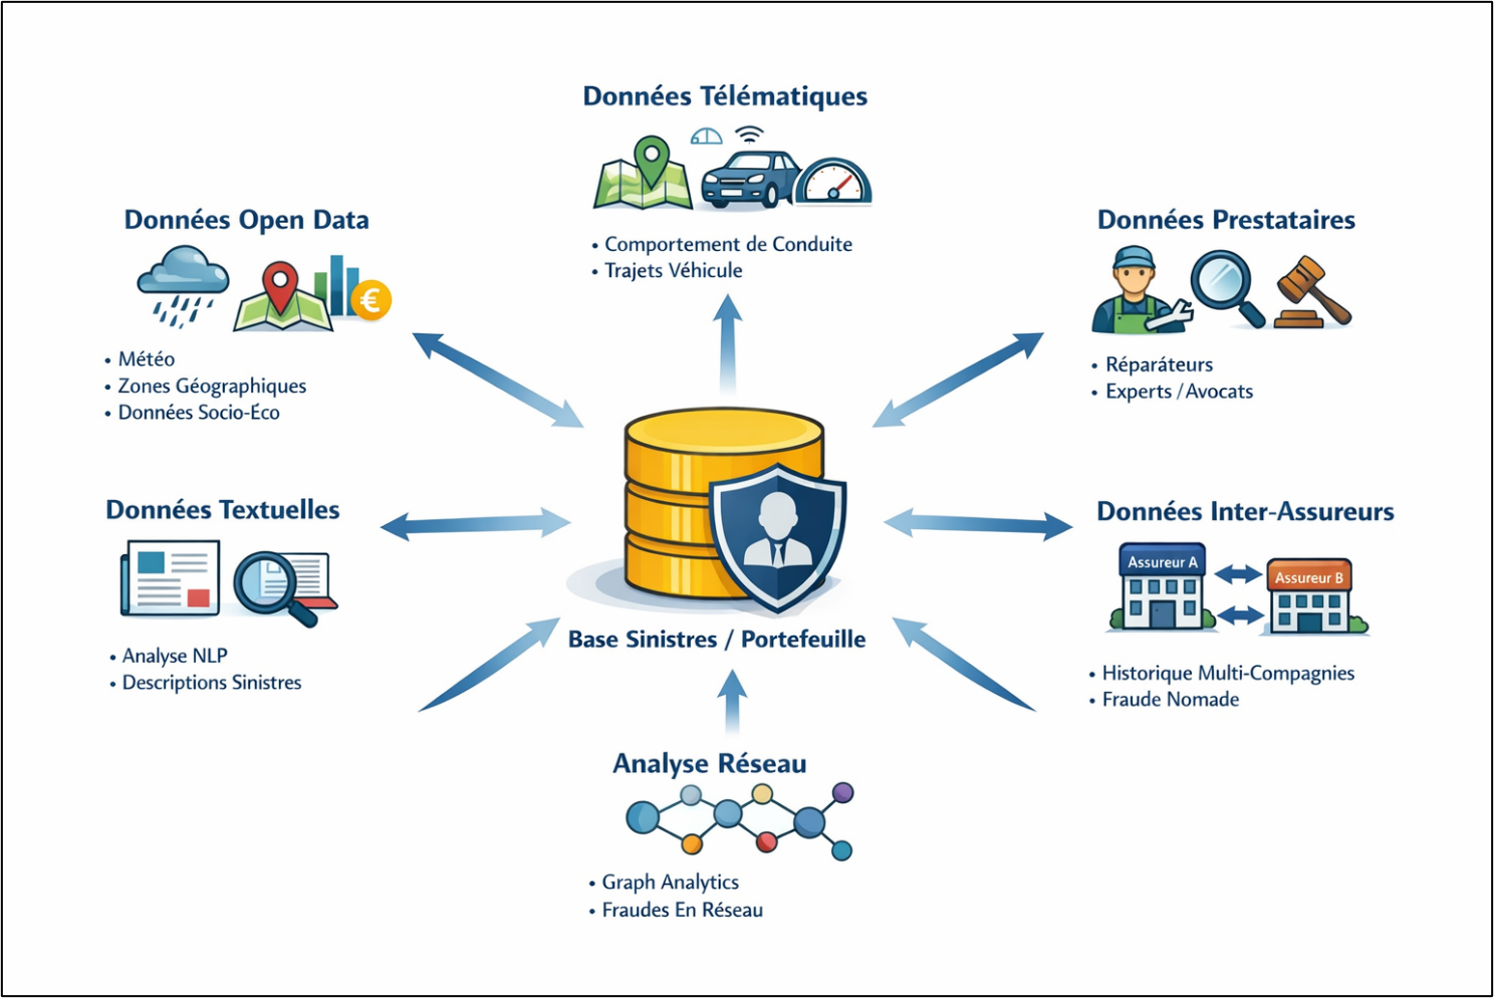
\includegraphics[width=0.85\textwidth]{images/chapitre7/couplage_sources_creation_agent.png}
    \caption{Couplage de sources de données pour la création de l'Agent de détection de fraude}
    \label{fig:couplage-sources}
\end{figure}

Ainsi, l'intégration de ces différentes sources de données permettrait de faire évoluer les modèles vers une approche plus globale, dynamique et contextualisée du risque de fraude, améliorant à la fois leur précision, leur robustesse et leur capacité à détecter des schémas complexes.

% --------------------------------------------------------------
\section{Mutualisation inter-assureurs et détection des fraudes organisées}
% --------------------------------------------------------------

Outre l'ajout de données externes, une piste d'amélioration majeure réside dans la \textbf{mutualisation des données et des outils entre assureurs}. En effet, les fraudes organisées reposent souvent sur des schémas répétés et peuvent concerner plusieurs compagnies. Un fraudeur détecté chez un assureur est susceptible de reproduire des comportements similaires auprès d'autres acteurs du marché.\footnote{https://www.ccomptes.fr/fr/publications/la-fraude-aux-cartes-grises}

Le partage d'informations, dans un cadre réglementaire maîtrisé, permettrait d'améliorer les \textbf{taux de détection des fraudes en bande organisée}, en identifiant plus rapidement des schémas récurrents et des profils à risque. Un agent IA alimenté par une base mutualisée bénéficierait ainsi d'une \textbf{vision élargie}, renforçant significativement son efficacité.

Un cas emblématique de fraude automobile organisée en France concerne le détournement du système d'immatriculation des véhicules (SIV), mis en place en 2017. Des réseaux ont exploité la possibilité, offerte aux professionnels habilités de réaliser des démarches administratives, en créant des « garages fictifs » servant de sociétés écrans. Ces structures ont permis l'immatriculation massive de véhicules frauduleux, facilitant notamment la réintroduction de véhicules volés dans le circuit légal et la dissimulation de leur traçabilité.\footnote{\url{https://www.ccomptes.fr/fr/publications/la-fraude-aux-cartes-grises}}

Selon plusieurs enquêtes de presse et sources sectorielles, cette fraude concernerait jusqu'à un million de véhicules et représenterait plus de 500 millions d'euros de pertes. Certains cas individuels font état de plusieurs milliers de véhicules immatriculés frauduleusement via une seule entité.

Ce type de fraude peut être qualifié de fraude en bande organisée dans la mesure où il repose sur une coordination de plusieurs acteurs aux rôles complémentaires : création de sociétés fictives, obtention d'habilitations administratives, production de documents frauduleux et utilisation répétée du dispositif à grande échelle. La structuration du schéma, son caractère durable dans le temps ainsi que les volumes traités témoignent d'une organisation planifiée et non d'initiatives individuelles isolées.

Bien que cette fraude ne cible pas directement un assureur en particulier, elle a des répercussions significatives sur l'ensemble du secteur de l'assurance automobile, en complexifiant la gestion des sinistres et en facilitant des fraudes secondaires. Ce type de schéma illustre le caractère structuré et organisé des fraudes de grande ampleur dans le domaine automobile.\footnote{Sources : \url{https://questions.assemblee-nationale.fr/q17/17-4793QE.htm} ; \url{https://www.senat.fr/questions/base/2025/qSEQ250102893.html}}

% --------------------------------------------------------------
\section{Extension à une approche multi-produits}
% --------------------------------------------------------------

Enfin, l'approche développée pourrait être étendue à une analyse transverse des comportements de fraude tous produits confondus. En effet, un individu impliqué dans une fraude en assurance automobile peut présenter un risque accru de fraude sur d'autres lignes de produits, telles que l'assurance habitation (MRH).

Une vision consolidée du client à travers l'ensemble des garanties permettrait de mieux capter ces comportements et d'améliorer la cohérence globale de la détection.

Cette approche multi-produits s'inscrit dans une logique actuarielle de \textbf{vision client 360°}, encore peu exploitée mais porteuse de gains significatifs en matière de lutte contre la fraude.

\subsection*{Conclusion}
\addcontentsline{toc}{section}{\textbf{Conclusion}}

Ce mémoire avait pour objectif de concevoir un outil d'aide à la décision permettant de détecter la fraude en assurance automobile et d'orienter les efforts d'investigation vers les dossiers les plus à risque. Il visait ainsi à répondre à une difficulté structurelle de la lutte anti-fraude : le coût d'une investigation manuelle, qui rend non rentable le contrôle de la fraude de faible montant et laisse échapper une part importante du préjudice. L'enjeu était donc de montrer qu'un agent d'intelligence artificielle pouvait automatiser cette détection à moindre coût et à grande échelle.

Pour y parvenir, il a d'abord fallu constituer une base de travail réaliste. Faute de données réelles suffisamment riches, nous avons enrichi une base publique de sinistres automobiles de trente variables simulées, reproduisant l'information dont dispose réellement un assureur au moment d'un sinistre (historique de l'assuré, du réparateur, du véhicule et du tiers, comportement déclaratif). Ce choix, assumé comme une limite, a permis de rapprocher l'exercice des conditions opérationnelles réelles.

La démarche s'est ensuite structurée autour d'un agent piloté par un prompt décomposé en étapes successives, reproduisant la logique actuarielle : ingestion et audit de la qualité des données, analyse statistique descriptive, puis construction et comparaison des modèles. Trois modèles ont été calibrés puis évalués selon un arbitrage entre interprétabilité et performance : un scoring en points, un arbre de décision et un modèle de Gradient \textit{Boosting}. Ce dernier s'est révélé le plus discriminant, sans toutefois disqualifier le scoring en points, qui demeure une alternative crédible lorsque la transparence prime. Nous avons par ailleurs constaté que les trois modèles faisaient converger leur pouvoir explicatif vers les mêmes variables clés, ce qui a renforcé la confiance dans la cohérence des résultats avec l'intuition métier.

L'un des partis pris forts de ce travail a été de décliner l'outil en deux modules indépendants, pensés pour deux profils d'utilisateurs distincts. Le premier, destiné aux actuaires, prend en charge la construction et la calibration du modèle ; le second, destiné aux gestionnaires de sinistres, en permet l'exploitation quotidienne sans en exposer la complexité, en restituant pour chaque dossier une probabilité de fraude et une orientation d'investigation. Cette séparation des rôles répond à une réalité de terrain : ceux qui conçoivent le modèle et ceux qui l'utilisent ne sont pas les mêmes équipes. Enfin, l'outil a été pensé non comme un modèle figé mais comme un dispositif évolutif : une boucle de rétroaction réintègre dans la base d'apprentissage les dossiers dont l'investigation est close, permettant un recalibrage régulier sur des cas avérés, tandis qu'un rapport de pilotage mesure en continu la valeur ajoutée de l'outil (fraude évitée, impact sur le ratio Sinistres/Primes, retour sur investissement).

Ce travail comporte naturellement des limites. La principale tient au caractère partiellement simulé des données et à la sur-représentation de la fraude dans la base retenue, qui imposeraient de recalibrer le modèle sur une sinistralité réellement représentative avant tout déploiement. Par ailleurs, l'approche supervisée adoptée ne détecte que la fraude de type connu, celle dont on possède des exemples historiques labellisés ; elle reste par construction aveugle aux schémas de fraude organisée ou inédits. Plusieurs prolongements permettraient de dépasser ces limites : le couplage à une base portefeuille, l'intégration de données externes, le recours à des méthodes non supervisées ou d'analyse de graphes pour la fraude en réseau, la mutualisation inter-assureurs pour repérer les fraudeurs « nomades », ou encore l'extension de l'outil à d'autres branches de l'assurance non-vie.

Au-delà de la seule performance technique, ce mémoire illustre la place croissante de l'actuaire dans la conception d'outils décisionnels concrets, à l'intersection de la modélisation, de la contrainte réglementaire et de l'usage métier. La détection de la fraude est devenue un enjeu stratégique pour les assureurs, et si l'intelligence artificielle en démultiplie aujourd'hui les moyens, elle ne prendra tout son sens qu'articulée à une supervision humaine garante de la maîtrise du risque et du respect des droits des assurés.
